%%%%%%%%%%%%%%%%%%%%%%%%%%%%%%%%%%%%%%%%%
% Minimalist Book Title Page 
% LaTeX Template
% Version 1.0 (27/12/12)
%
% This template has been downloaded from:
% http://www.LaTeXTemplates.com
%
% Original author:
% Peter Wilson (herries.press@earthlink.net)
%
% License:
% CC BY-NC-SA 3.0 (http://creativecommons.org/licenses/by-nc-sa/3.0/)
% 
% Instructions for using this template:
% This title page compiles as is. If you wish to include this title page in 
% another document, you will need to copy everything before 
% \begin{document} into the preamble of your document. The title page is
% then included using \titleTH within your document.
%
%%%%%%%%%%%%%%%%%%%%%%%%%%%%%%%%%%%%%%%%%

%----------------------------------------------------------------------------------------
%	PACKAGES AND OTHER DOCUMENT CONFIGURATIONS
%----------------------------------------------------------------------------------------

\documentclass{report}

\usepackage[svgnames]{xcolor} % Required to specify font color
\usepackage{graphicx} %Required for images
\usepackage[nottoc,numbib]{tocbibind} %Include bib
\usepackage[babel, stor, nat, en, titelside]{ku-forside}  %Front page

%----------------------------------------------------------------------------------------
%	TITLE PAGE
%----------------------------------------------------------------------------------------

\titel{Bachelorprojekt 2014} %
\undertitel{Midtvejs-rapport} %
\opgave{Operating Systems - kUdOS} % Findes kun under 'titelside'
\forfatter{Philip Meulengracht - lpz849}%
\dato{22 April 2014}%
\vejleder{Jost Berthold} %  Findes kun under 'titelside'

%----------------------------------------------------------------------------------------
%	BLANK DOCUMENT
%----------------------------------------------------------------------------------------

\begin{document} 

\maketitle % Creates front page

%Add TOC

\tableofcontents

%Now, first page!

\newpage

%----------------------------------------------------------------------------------------
%	SURVEY
%----------------------------------------------------------------------------------------

\chapter{Background}

\section{Project Description}

In my thesis work, I want to improve the educational tools for teaching Operating System. In order to make an informed decision about design, I plan to survey existing educational operating systems, and evaluate their advantages and drawbacks. I will not be writing any tool or any program from scratch, I will take an already existing tool, or project as my base-line and work from that as a starting point.
The educational operating systems are operating systems that exists to show people how a minimalistic operating system functions, the most basic of a complex system.
The project I will take as a starting point will be the operating system Buenos, because it seems like Buenos has immense documentation that explains a lot about why, where and how the operating system functions without introducing too advanced concepts, so it is without a doubt very academic.
Buenos also demonstrates in its design decisions that it always takes the more academic route (with documentation and examples), instead of the faster, simpler route, which is a huge plus and in the spirit of this thesis. The problem - or the challenge - with Buenos is that it is currently not an integrated developing/testing solution, and it targets a platform that is more or less not widely used, and my goal is to add a lot more value to the project for the users. I think that Buenos would be much more interesting for students if it was actually targeting a more recent platform, and if I could make it into a more integrated solution, so you would not have to run a MIPS simulator in a virtual machine. While making these improvements to Buenos, I will produce high quality educational documentation.
I want to clarify the meaning of Integrated Solution in this case, because one the goals will be to reach something easier than the current solution, which is using a virtual machine, to use an emulator that can then virtualize the Buenos. I want to make a disk image, that dual boots Buenos and a small Linux development environment, where you can directly update the on-board Buenos boot with the newest build.

\pagebreak
\section{Survey}

I had two options for my project, either I would take an existing project and modify it to my requirements, or to code a new operating system from scratch. The sensible solution was to use an existing code base due to the amount of work that goes into such a project. I then researched the current available code-bases I could use, and it was easy to find almost 20 educational open source operating systems that could have been used as a basis, I however decided to discuss some of the more popular operating systems, which I have listed below.
The reason I've chosen these exact projects are due to their availability, extensive documentation and that they are mostly distinct operating systems.

\begin{itemize}
  \item Minix
  \item Nachos
  \item Pintos
  \item Buenos
\end{itemize}

\subsection{Minix}

Minix is the project of Andrew S. Tanenbaum, and is a part of his book\cite{AndrewTanenbaum} he wrote to demonstrate the principles of operating systems. The Minix operating system is written to be Unix-compatible and supports a variety of architectures. The original project, released in 1987\cite{MinixRef1}, was released as an educational operating system, and the following years as popular architectures changed, updated versions of Minix were released. The Minix 2.0 version was released in 1997, and the most noticeable difference between the original 1.1 version and 2.0 version was that Minix now supported the first generation of IBM computers, and support for various other architectures were implemented as well (SPARC, Motorola etc). In 2006 Minix 3.0 was released, and a lot of the core system remained unchanged, however all device drivers were now separated user-land processes and became truly independent.

Minix features\cite{MinixRef}:

\begin{itemize}
  \item Micro-kernel (Supports processes, multiple file-systems, many drivers)
  \item Supports x86-32
  \item Well-documented
  \item Already has exercises made
  \item Large, well-featured user-land
\end{itemize}
'
The list of features for Minix is extensive, and thus I won't go into a very detailed feature-list. For this reason I won't be using Minix for my project, since the project today is huge and it already has a lot of features. One thing that does stand out on this not-so-detailed feature list is that Minix is a micro-kernel.

There area few kernel design-concepts, and the typical design for a education operating system is a monolithic design, which means all kernel-services run in the kernel-land and is a part of the kernel, both file-systems and device drivers. The advantage of monolithic design is that it is very simple, and it works.
A micro-kernel has everything independent of each other, and generally the kernel just support processes, I/O access, MMU and a scheduler. Device drivers, file-system drivers and most services run separated in user-land. The advantage of this design is that it is very neat to deal with, and it has fault-tolerance, which means if a driver crashes, it can be restarted where it might have led to a system crash in a monolithic design. A micro-kernel also is a better design for security-oriented system due to the fact everything is separated and no device-drivers actually have any direct I/O access.

\subsection{Nachos}

Nachos was originally written in 1991 at Berkeley and was released in 1992. The project was maintained until 1996 and the Nachos 4.0 version is the last original version. Nachos is not directly a operating system, but rather a simple MIPS-simulator and then an operating system on top of that simulator which runs as a program. Nachos is a very limited project, and various successor projects have been started since its demise in 1996. Two people at Berkeley also attempted a version 5.0 which ran in Java in an effort to make it more available to students and easier to use as teaching material, however none of this was very optimal.

Nachos features\cite{NachosRef}:

\begin{itemize}
  \item Monolithic Kernel
  \item Supports multiple-threads, but only one at a time
  \item Processes
  \item Virtual file-system
  \item Interrupt Queue
  \item User-land with separated memory
  \item A built-in debugger
  \item Well-documented
  \item Already has exercises
\end{itemize}

The feature-list for nachos is not the most extensive, and this is simply because Nachos lacks a lot of features. Nachos instead comes with an empty framework, where many components are  meant as exercises. These exercises cover most of the operating system. Nachos lacks important features as synchronization between threads, system calls, simultaneous user programs, networking, a proper file-system and virtual memory management. While it is not a very bad idea to leave all of this to the students as exercises, I feel examples\footnote{Simple implementations} should be provided since there is in this case no accompanying book like Minix to describe the concepts.

I will not be using Nachos due to a few factors. For one it's not a dedicated kernel, but instead is a kernel built upon a simulator, which means that porting it to a sensible platform would be a huge project. Another problem is the fact that it is missing a file-system and a virtual memory manager, which would also has to be written. 

\subsection{Pintos}

Pintos was released in 2004 and was targeting a more popular architecture, the Intel x86-32. The project was originally started by Tom Anderson at Berkeley and was actually inspired by Nachos and maintains some of their concepts. Unlike Nachos, Pintos is a dedicated kernel and actually will run on real hardware\footnote{As stated in its road-map, it will \emph{in theory} run on real hardware}, even though it is preferred to run it in a simulator like Bochs, VirtualBox or QEmu.

Pintos features\cite{PintosRef}:

\begin{itemize}
  \item Monolithic Kernel
  \item Supports x86-32
  \item Supports multiple-threads
  \item Processes
  \item Virtual file-system
  \item Virtual Memory
  \item User-land, System calls
  \item Unix-like file-system
  \item Debugging tools
  \item Well-documented
  \item Already has exercises
\end{itemize}

Pintos has a typical feature-list for an educational operating system. It has a monolithic design and supports the features as threads, processes, a file-system, virtual memory manager and system calls. Pintos contains very simple implementations of the mentioned components which is an huge advantage for an educational operating system.
After going through the documentation about Pintos it becomes clear how it resembles Nachos, large parts of each component is missing and left as exercises to the students. Pintos leaves threads, user programs, file-system and virtual memory as exercises. Unlike Nachos, Pintos however is a better candidate for a project due to a few reasons. Pintos is not completely missing the aforementioned parts, it does have very minimal and simple implementations of these components. Pintos also targets an architecture which does not need to be emulated, but is of course easier with emulation.

\subsection{Buenos}

Buenos is a small multi-core operating system and is currently used for teaching at University of Copenhagen. Buenos was released back in 2003 together with YAMS, which is the accompanying MIPS-simulator. The unique thing about Buenos is that it is an SMP operating system skeleton. Buenos is hardly still maintained and could use an overhaul of some of its systems. It also lacks a few important components, and does not support multiple user-processes.

Buenos features\cite{BuenosRef}:

\begin{itemize}
  \item Monolithic Kernel
  \item SMP (Multi-core)
  \item Multi-threading
  \item Strong synchronization
  \item Single user-process
  \item Virtual file-system
  \item User-land, System calls
  \item Simple file-system
  \item Well-documented
  \item Already has exercises
\end{itemize}

The advantage of Buenos is that it is a SMP operating system and natively support multi-core, and the framework is built with SMP in mind. Buenos has strong synchronization for this purpose with semaphores, spin-locks and sleep queues. The feature-list is lacking some important components, or some capability in terms with user processes. Buenos has no dynamic memory allocation and only supports one user process at the time, which is not typical considering it has proper multi-threading. Another drawback Buenos is possessing is that it only runs on MIPS architecture, which must be simulated. However Buenos is a really great candidate, since the implementation it provides are simple, most of the code is easily portable, it has its very own file-system and it is very well documented in its Road-map. 

\subsection{Conclusion}

The four different operating systems, Minix, Nachos, Pintos and Buenos all had their advantages and disadvantages. Minix had every feature you could dream of in an educational operating system which also made it impractical to use for my project, since I am looking to improve an existing educational operating system instead of writing a new from scratch, which would be too much work for a bachelor-thesis, and I see no simple exercises or simple concepts to improve in Minix.

Nachos could have been a good project, but it lacked some important components, and furthermore it would require a lot of work to port it to x86 architecture since it's built directly for the included MIPS simulator.

Pintos could also have been a great candidate for my project, it already targets the x86 architecture and provided minimal and simple implementations of most components, but I could not spot enough work in the project, I would only have to extend the current implementations and provide dynamic memory allocation examples.

The last project, Buenos seems to hit a sweet-spot between work needed and convenience. Buenos needs to be ported to the x86 architecture, and also needs work done in its memory components, but unlike Nachos a lot of the code in Buenos is actually portable enough\footnote{Barely portable enough} so the project will be far from as extensive as Nachos. The convenience in using Buenos is that the University of Copenhagen is already using this operating system for teaching, and thus it would be a lot easier to use the improved Buenos as its concepts would remain the same, and no special modifications would be needed in the course.

I will be changing the name of the operating system due to the amount of modifications needed, and I will be referring Buenos to kUdOS for the rest of the report.

%----------------------------------------------------------------------------------------
%	DESIGN
%----------------------------------------------------------------------------------------
\newpage
\chapter{Design Choices}

\section{Technical Choices}

In order to get started on my project I had to make a few technical decisions about the direction the project should take. The first decision I had to make was which architecture I wanted to port the operating system to, and the second choice I had to make was if I were going to use an existing boot-loader, or write my own (which might be a better choice depending on target architecture).

\subsection{Target Architecture}

When I started writing my project, I wanted to port kUdOS to the Intel x86-32 bit architecture, simply because it is the most mainstream architecture and there are many advantages as to why you would want to teach operating systems with that architecture. The primary advantage of picking the x86 architecture is due to the information, tutorials, emulators and examples available. 

As I progressed with my project it became obvious that I might as well target the x86-64 bit architecture because I was going to implement multi-core. I realized this because that it simplifies a lot of x86 architecture code due to the requirements for a x86-64 bit CPU. A 64 bit CPU must support an APIC\footnote{Advanced Programmable Interrupt Controller (APIC), this is the replacement for the PIC (Programmable Interrupt Controller). The PIC is in newer computers obsolete and typically emulated for legacy purposes by the APIC. The PIC controls the interrupt-lines from hardware-devices, and is programmable by software so a Kernel can decide how to map callback-functions to each interrupt-line.}, it also must support a few other CPU feature extensions that simplifies initialization setup. There is also no extra complications by choosing 64 bit over 32 bit, it only requires me to setup paging a little different than otherwise.

\subsection{Boot-loader}

This decision was easy for me, I do not have the resources or the time to write a custom boot-loader for kUdOS, even though it would be very educational to do so. Instead I went with the more sane and easy solution, to use an existing open source boot-loader, that is capable of multi-booting and booting x86 kernels.

There exists a few open source boot-loaders on the Internet that is capable of booting kernels on the x86 architecture, which can do all the basic initialization of a system, load a kernel and call the kernel entry-point. This simplifies the booting process and makes sure we can focus on what is important, the operating system itself. 
My goal is to have an integrated developing solution, that contains both a stripped Linux distribution for development, and an on-board kUdOS installation so it would be possible to boot directly into kUdOS. This meant that since we will be having a Linux distribution, we will have GRUB already installed as a boot-loader. GRUB actually match my requirements for a boot-loader, it can multi-boot, load x86 kernels, is open source and free to use, so I decided to go with GRUB.

\section{Project Layout Changes}

The current layout of the project was not fit for multiple architectures and generally didn't split up the code as effective as you might think by a first look at the project directory-structure.

\begin{figure}[h]
    \centering
    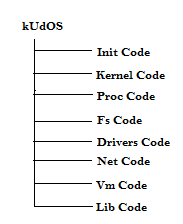
\includegraphics{DirectoryLayoutBegin.png}
    \caption{kUdOS Project Layout}
    \label{fig:code_layout_end}
\end{figure}

All the platform-dependent code is mixed up with the platform-independent code within these sub-directories. I had a few options that concerned splitting the platform-depending code from the platform-independent code, I could either make a new directory called \emph{Arch} and make a sub-directory within this folder for each architecture supported like illustrated below.

\begin{figure}[h]
    \centering
    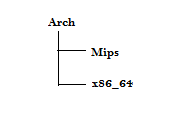
\includegraphics{LayoutProposal1.png}
    \caption{kUdOS Project Layout Example 1}
    \label{fig:code_layout_ex1}
\end{figure}

However, the problem with this method of splitting source-code was because of the way the current Makefile was constructed, which is to have a sub-makefile in each directory that contains each source-file to be compiled. I tried to do it this way the first time, but had a lot of complications making it transparent to the user/student of the project, primarily because I was forced to do a lot of if/then/else switches both in code and the Makefile, which I wanted to avoid. I then came up with a second way to structure the layout of the project to make it transparent and have the code separated.

\begin{figure}[h]
    \centering
    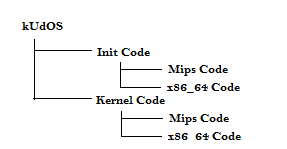
\includegraphics{LayoutProposal2.png}
    \caption{kUdOS Project Layout Example 2}
    \label{fig:code_layout_ex2}
\end{figure}

With this structure it was easier to modify the Makefile to support multiple compilation-targets. The advantage of this layout was that this also kept the separated platform-dependent code categorized. With the project layout re-distributed and the Makefile changed to reflect these modifications, it suddenly become a lot easier to support both the MIPS and the x86 architecture. Aside from the directory-structure changes to the platform-dependent code I have not made any changes. I've tried to keep it as original as possible.

%----------------------------------------------------------------------------------------
%	PROJECT PROGRESS
%----------------------------------------------------------------------------------------
\newpage
\chapter{Project Progress}

\section{Setup}

As I described in my project description, one of my goals with kUdOS is to provide developers/students with an integrated solution, where they would be able to dual-boot a Linux distribution that is set-up as a developer environment, and a direct boot option for kUdOS, and this would be my top priority for the start of this project. I also created a virtual machine in VirtualBox and installed a stripped\footnote{I removed every application that wasn't related to developing or suited for my use} Ubuntu distribution. In this Ubuntu I have compiled cross-compilers for both the MIPS and x86-64 architecture. The second step of creating this integrated environment was to make sure I had enough partitions on my virtual hard-drive image, I had to use 2 partitions for the Ubuntu\footnote{1 partition for Ubuntu, 1 for Swap} distribution, and 2 extra partitions for my on-board kUdOS\footnote{1 Fat32 for the kernel image, 1  raw partition for kUdOS own file-system} installation. I also installed Bochs and YAMS as virtual machines for testing both the MIPS and x86-64 kernels without having to reboot my virtual machine. The final step was then to prepare the kUdOS source-code and make sure it compiled and ran in YAMS, so I had a starting point.

\section{Layout Changes}

The source-code layout that was present in the kUdOS project directory was not suited for having multiple architectures. The source-code was split up into a few sub-directories which each explained their use.

\begin{figure}[h]
    \centering
    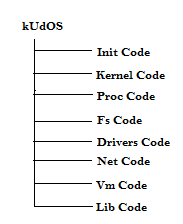
\includegraphics{DirectoryLayoutBegin.png}
    \caption{kUdOS Source-Code Layout}
    \label{fig:code_layout_end}
\end{figure}

This is simple, but fine directory-layout if you only want to target a single architecture, which probably was the first intentions with Buenos (now, kUdOS). So to make kUdOS multi-architecture friendly, I wanted to separate all architecture-specific code from the independent and higher layers of the system. I took every sub-directory that had architecture-specific code and put it into its respective architecture sub-folder. After I had modified the layout it now looked like this

\begin{figure}[h]
    \centering
    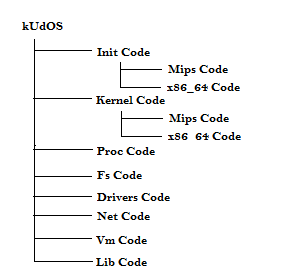
\includegraphics{DirectoryLayoutEnd.png}
    \caption{kUdOS Source-Code Layout}
    \label{fig:code_layout_end}
\end{figure}

This way I could also keep the Makefile structure and simply control everything from the main Makefile, simply by just adding the new build to the Makefile.

\section{Porting to X86-64 Architecture}

In order to port the kernel from the MIPS architecture to the x86-64 architecture, I had to plan out which initialization steps I had to go through to achieve a common entry-point for both the Mips and x86-64 kernel.

As mentioned earlier I decided to use GRUB as the boot-loader\footnote{GRUB handles basic computer initialization and loads a kernel image into memory, and executes from the image's entry point. It supports multi-boot.} for the x86-64 kernel instead of writing my own (for many, many reasons), since it came with the Ubuntu installation, and is the default boot-manager in Linux. GRUB uses the multi-boot specification for booting non-Linux kernels, and kUdOS will not be a Linux kernel, so I will conform to the multi-boot specification.

The multi-boot specification requires us to have a custom multi-boot header located in the first 8 kilobyte of the kernel image, and requires the kernel format to be either of raw binary or of the ELF\footnote{It's the default executable-format in Linux.} format. In this multi-boot header we specify how we want GRUB to initialize the system before handing control to our kernel.

\begin{verbatim}
MultibootHeader:
	.long 0x1BADBOO2			/* Multiboot Magic Number */
	.long 2				/* Flags */
	.long (0x1BADBOO2 + 2)		/* Checksum */
\end{verbatim}

The above I have put in the initialization assembly file that contains our entry-point, and I wrote a linker script for GCC to use to make sure that the above code ended up in the first 8 kilobytes of the kernel image. It is the most basic of the multi-boot header and thus GRUB does no special further initialization except the basics and then passes control to our entry point. To make sure GRUB could see kUdOS I had to modify the GRUB-configuration file and re-update GRUB.

Next I researched what steps must be done in order to initialize 64 bit mode (also known as long mode) in x86. In order to do so I had to follow these steps.

\begin{itemize}
  \item Disable Interrupts while doing initialization
  \item Make sure the CPU supports long-mode
  \item Load the 32 bit Global Descriptor Table\footnote{The Global Descriptor Table (GDT) describes the different memory selectors, it is primarily used for memory segmentation, but in our case there will be 5 descriptors, a Null descriptor (must exist), 2 kernel descriptors (1 Code descriptor, 1 Data descriptor) and 2 user-mode descriptors (1 Code, 1 Data). The last 4 covers all memory because we will not be using segmentation.}
  \item Initialize a PML4 Page Directory and load it
  \item Load the 64 bit Global Descriptor Table
  \item Jump to 64 bit mode
\end{itemize}

All of these steps must be done in assembly, due to the fact that we must be able to control every single detail and aspect of the initialization process. I wrote these into the file \_boot.S which contains the primary initialization process of x86-64 bit, and after entering 64 bit mode I call an entry point in C-code, switching away from assembly. I closely follow the above steps, by setting up the GDT for both 32 bit and 64 bit mode, and setting up a PML4 Page Directory. 

The x86 architecture makes use of virtual memory, and the MMU\footnote{Memory Management Unit} handles the translation of virtual memory addresses to physical memory addresses with a Page Directory. In 32 bit architecture we only have a single page directory, which can map 4 gigabytes of memory. The page directory has 1024 page tables, and each page-table has 1024 page entries. Each page maps 4096 bytes (4KB). This means that each page table can map 4 megabytes of memory, and thus 1 page directory maps 4 gigabytes of memory. When we look at the 64 bit architecture, this naturally becomes insufficient, since with 64 bit memory addresses, you can access a lot more than just 4 gigabyte, and thus we need something larger than a page directory. In 64 bit the PML4 page directory table gets introduced, and has 512 page directory entries, and each page directory has 512 page-table entries, and each page-table has 512 pages. Each page can map either 4 KB or 2 MB, depending on the page-flags (this applies to 32 bit as well, when 2 MB pages are used, you are able to access more memory using PAE\footnote{Physical Address Extension}).

After making the jump into long mode, we cease to use assembly for a little while and can now enter the world of C-programming.

%----------------------------------------------------------------------------------------
%	FUTURE STEPS
%----------------------------------------------------------------------------------------
\newpage
\chapter{Next steps}

\section{Memory Manager}

Both the physical and virtual memory manager is the next primary step I have to make in my project. The current memory manager is directly tailored to the MIPS architecture, and currently only supports 32 bit memory addresses. I want to give the physical memory manager the ability to handle 64 bit memory addresses when compiled for the 64 bit architecture, and keep the 32 bit capability when compiled for MIPS, since it would be a waste of memory if we kept the 64 bit capability for a 32 bit physical memory manager.

For the virtual memory manager it becomes more complex, since the paging systems vary a lot from the 64 bit Intel architecture and the 32 bit MIPS architecture. In this case I will have to be creative by either keeping the current virtual memory manager and writing a new for the x86-64 platform, or see if it will be possible to somehow make the two different memory managers transparent and support both systems. It probably will be complicated due to the difference in address sizes.

Currently kUdOS does not have a heap memory manager\footnote{Implements support for dynamic memory allocation}, however I, if time permits, will try to write a simple implementation of a linked-list heap manager to allow for dynamic memory allocation through the use of kmalloc/kfree. An possible exercise for students could then be to either extend this heap manager, or to write a new, more complex/efficient heap manager.

\section{Driver System}

The driver system currently is not abstract enough to support both the x86 architecture and the MIPS architecture. Even the platform-independent code seems somewhat tailored to the MIPS architecture and thus will need rewriting, and will be the first step. When the driver system is more abstract and capable of supporting both architectures, I will write the necessary x86 drivers that will be needed for the kernel. The needed drivers will be:
\begin{itemize}
 \item Global Descriptor Table Driver
 \item Interrupt Descriptor Table Driver
 \item Exceptions Driver
 \item APIC Driver
 \item CPU Driver
 \item AP\footnote{Application Processor (AP), this is the extra cores. The x86 architecture only starts 1 core, not all of them. You have to start the other cores manually.} Driver
\end{itemize}

\section{Updating Road-map}

This step is something I will do gradually as I progress through my project, I will reflect the modifications to the project in this Road-map, both project name changes, the project layout changes and the changes done to both the driver system and memory manager. A lot of the information will have to be changed in order to reflect that kUdOS has become multi-platform and the interfaces become more abstract. 

%----------------------------------------------------------------------------------------
%	LITTERATURE
%----------------------------------------------------------------------------------------

\begin{thebibliography}{9}

\bibitem{AndrewTanenbaum}
  Andrew S. Tanenbaum,
  \emph{Operating Systems: Design and Implementation}.
  Prentice Halls,
  First Edition,
  1987.

\bibitem{MinixRef}
  Minix Specifications,
  \emph{http://www.minix3.org/}
  Specifications \& About Minix.

\bibitem{MinixRef1}
  Minix History,
  \emph{http://www.cs.vu.nl/\~ast/brown/}
  History \& About Minix.

\bibitem{NachosRef}
  Nachos Specifications,
  \emph{http://homes.cs.washington.edu/\~tom/nachos/}
  Road-map \& About Nachos.

\bibitem{PintosRef}
  Pintos Specifications,
  \emph{http://www.stanford.edu/class/cs140/projects/pintos/pintos.html}
  Road-map \& About Pintos.

\bibitem{BuenosRef}
  Buenos Specifications,
  \emph{http://www.niksula.hut.fi/\~buenos/buenos.html}
  Road-map of Buenos.

\end{thebibliography}

\end{document}
